\documentclass[]{scrartcl}
\title{Vorlesung Analysis II}
\usepackage{amsmath,amssymb,amsfonts}
\usepackage{stmaryrd}
\usepackage{mathtools}
\usepackage{latexsym}
\usepackage{graphicx}
\usepackage{tikz}
\usepackage{xcolor}
\usepackage[most]{tcolorbox}
\usepackage{soul}
\usepackage{ upgreek }
\usepackage{hyperref}
\usepackage{tipa}
\usepackage[dvipsnames]{xcolor}
\hypersetup{
	colorlinks=true,
	linkcolor=blue,
	filecolor=magenta,      
	urlcolor=cyan,
	pdftitle={Overleaf Example},
	pdfpagemode=FullScreen,
}
\newcommand{\redcircle}[1]{%
	\tikz[baseline=(char.base)]{
		\node[shape=circle, draw=red, text=red, thick, inner sep=1pt] (char) 
		{\textbf{#1}};
	}%
}
\newcommand{\bluecircle}[1]{%
	\tikz[baseline=(char.base)]{
		\node[shape=circle, draw=blue, text=blue, thick, inner sep=1pt] (char) 
		{\textbf{#1}};
	}%
}
\newcommand{\blackcircle}[1]{%
	\tikz[baseline=(char.base)]{
		\node[shape=circle, draw=black, text=black, thick, inner sep=1pt] 
		(char) 
		{\textbf{#1}};
	}%
}
\newcommand{\orangecircle}[1]{%
	\tikz[baseline=(char.base)]{
		\node[shape=circle, draw=orange, text=orange, thick, inner sep=1pt] 
		(char) 
		{\textbf{#1}};
	}%
}
\newcommand{\redul}[1]{\setulcolor{red}{\ul{#1}}}
\newcommand{\blueul}[1]{\setulcolor{blue}{\ul{#1}}}
\newcommand{\yelul}[1]{\setulcolor{yellow}{\ul{#1}}}
\newcommand{\greenul}[1]{\setulcolor{green}{\ul{#1}}}
\newcommand{\oraul}[1]{\setulcolor{orange}{\ul{#1}}}
\setul{1pt}{1.5pt} % Linienhöhe und Abstand zum Text (optional anpassbar)

\setlength{\topmargin}{-.5in} \setlength{\textheight}{9.25in}
\setlength{\oddsidemargin}{0in} \setlength{\textwidth}{6.8in}
\setlength{\parindent}{0pt}

\begin{document}
	\maketitle
	\textbf{\underline{Teil 3: Gewöhnliche Differentialgleichungen}}\\
	\\
	\textbf{\underline{an 23: Differentialgleichungssysteme}}\\
	\\
	\textbf{\underline{\underline{Stichworte:} DGLsysteme (Linear 1. ordnung, Konstante Koeff.), Jordan-Normalform}}\\
	\\
	\textbf{\underline{Literatur:}} frühere Vorlesung in \blueul{Lineare Algebra II, Kapitel l 14.}\\
	\\
	\textbf{23.1. \underline{Einleitung:}} Wir lösen DGLsysteme 1. Ordnung (Linear mit Konstanten Koeffizienten) durch Anwenden des Satzes von dder Jordan-Normalform aus der Linearen Algebra II.\\
	\\
	\textbf{23.2. \underline{Motivation:}} Manche DGLn, etwa Lineare höhere Ordnung, lassen sich in DGLsysteme umformen und in Matrixform bzw. mit Funktionen bestehend aus mehreren Komponenten Kurzgefasst notieren und Lösen.\\
	\\\textbf{23.3. \underline{Vereinbarung:}} $y:\mathbb{R}\rightarrow\mathbb{C}^n$, \yelul{y(x)=}$\begin{pmatrix}
		y_1(x)\\
		y_2(x)\\
		\vdots\\
		y_n(x)
	\end{pmatrix}$ sei eine Funktion auf $\mathbb{R}$ (der Zeit x) die Komponentenfunktionen $y_1,...,y_n$ seien stetig diff'bar.\\
	dazu sei $y':\mathbb{R}\rightarrow \mathbb{C}^n, \ x\rightarrowtail y'(x):=\begin{pmatrix}
		y_1(x)\\
		y_2(x)\\
		\vdots\\
		y_n(x)
	\end{pmatrix}$ die Ableitung. Sie ist stetig auf $\mathbb{R}$.\\
	Weiter sei \yelul{A:=$(a_{ij})$}$\in\mathbb{C}^{n\times n}$ eine fest gewählte n x n- Matrix.\\
	\\
	\textbf{23.4. \underline{Bezeichnung:}} (i) Wir nennen eine Abb. $D:y\rightarrowtail$\yelul{D(y)}:=\redul{y'-Ay},\\
	d.h. $(D(y))(x):=y'(x)-A\cdot y(x)$,\\
	einen \redul{Linearen Differential-Operator erster Ordnung mit Konstanten Koeffizienten.}\\
	(ii) Für eine stetige Funktion $b:\mathbb{R}\rightarrow \mathbb{C}^n, \ \rightarrowtail b(x):=\begin{pmatrix}
		b_1(x)\\
		\vdots\\
		b_n(x)
	\end{pmatrix}$\\
	heißt \fcolorbox{red}{white}{D(y)=b}, d.h. \fcolorbox{red}{white}{y'=Ay+b} ein \redul{Lineares Differentialgleichungssystem $\underbrace{\text{erster Ordnung}}_{\rightarrow\text{d.h. maximal erste Ableitung kommen vor}}$ ($\underbrace{\text{mit Konstanten Koeffiziente}}_{\text{die Einträge von A sind Konstant, d.h. keine Veränderlichen Funktionen in x}}$n)}.\\
	Ist b(x)$\equiv$0 (konstant-0-Fkt.) so reden wir von einem \redul{homogenen System}, sonst von einem \redul{inhomogenen System}.\\
	\\
	\textbf{23.5. \underline{Bem.:}} Haben $D\in \ Hom(\varphi^1(\mathbb{R},\mathbb{C}^n), \varphi^0(\mathbb{R},\mathbb{C}^n))$ als Homomorphismus zwischen Funktionenräumen (sind ja $\mathbb{R}-VRe$) was die Benennung "linearer Differentialoperator" rechtfertigt. In der Funktionalanalysis heißen Abb.en zwischen Funktionsräumen \redul{Operatoren}.\\
	\\
	Die Struktur der Lösungsmenge erhält man aus der Linearen Algebra I:\\
	\textbf{23.6. \underline{Lemma:}} Ist \greenul{$y_p$ (irgend)eine (partikuläre/spezielle) Lösung} des inhomogenen Systems  Dy=b, d.h. von y'-Ay=b, so ist \redul{$\mathbb{L}(D;b):=\{y_p+y_H;\ y_H \in ker \ D\}$} die \greenul{Gesamtheit aller Lösungen}.\\
	Dabei besteht \greenul{ker(D)} aus allen \greenul{Lösungen der homogenen Gleichung $Dy_H=0$},\\
	d.h. 
	von $y_H'-Ay_H=0.$\\
	\underline{Bew.:} Vgl. Vorl. zur \blueul{LA I}, bzw. \oraul{$y\in\mathbb{L}(D;b)\Leftrightarrow y-y_p\in\ ker(D)=D^{-1}(\{0\})$}.\\
	\strut\hfill$\square$\\
	Die homogene Gleichunge hat folgende Eigenschaft.\\
	\textbf{23.7. \underline{Lemma:}} Ist y Lösung von $D_=0$, d.h. ist \greenul{y'=Ay} (d.h. ist homogene Lsg.),\\
	und ist $x_0 \in \mathbb{R}$ eine Nullstelle von y, d.h. \greenul{$y(x_0)=0$},\\
	so ist \greenul{y(x)=0 für alle $x\in\mathbb{R}$}, d.h. y(x)$\equiv$0 Konstant =0.\\
	\underline{Bew.:} Für jedes $t\in\mathbb{R}$ ist $y'(t)=Ay(t)$, so dass \oraul{$y_i'(t)=\sum_{j=1}^{n}\alpha_{ij}y_j(t)$}\\
	Durch Integration folgt\\
	\oraul{$y_i(x)=y_i(x_0)+\int_{x_0}^{x}y_i'(t)dt=0+\int_{x_0}^{x}\alpha_{ij}y_j(t)dt$}.\\
	mit \oraul{$\eta(x):=\max\{ \max\{|y_i(t); \text{für t mit }|t-x_0|\leq|x-x_0|\};\ i=1,...,n\}$} und \oraul{a:= $\max\{|\alpha_{ij}|;\text{alle }i,j\}$} ist damit\\
	\oraul{0$\leq \eta(x)\leq$} $\int_{x_0}^{x}n\cdot a \cdot a \cdot \eta(t)dt \leq \eta (x)\cdot n\cdot a \cdot |x-x_0|.\\$
	Ist x so nahe bei $x_0$, dass \oraul{$na|x-x_0|\textless 1$}, folgt daraus notwendig \oraul{$\eta(x=0)$}, also auch $\eta(t)=0$ für $|t-x_0|\textless|x-x_0|.$\\
	Dieser Schluss ist $\underbrace{\text{iterierbar}}_{erst: y(x)=0 \textbf{für alle x nahe }x_0\text{, dann alle x(induktiv) erreichbar...}}$\\
	\strut\hfill$\square$\\
	\textbf{23.8. \underline{Folgerung:}} (i) Für \greenul{jedes $y_0 \in \mathbb{C}^n$}, hat das \greenul{Anfangswertaufgabe Dy=b, y(0) $\overset{!}{=} y_0$}, \greenul{höchstens eine Lösung}.\\
	(ii) Die Abbildung \greenul{$\varphi: \ ker D\rightarrow \mathbb{C}^n,\ y\rightarrowtail y(0)$},\\
	ist \greenul{injektiv}, und damit ist \greenul{dim ker D $\leq$ n}.\\
	\\
	\textbf{23.9. \underline{Bem.:}} Tatsächlich gibt es bei (i) stets eine Lösung, dann also eindeutig. Denn: Mit \blueul{23.10.} sehen wir, dass \greenul{$\varphi$ bijektiv} ist und dann \greenul{dim ker D=n} ist.\\
	\underline{Bew.:} (i): Sind $y_1,y_2$ Lösungen von Dy=b, jeweils mit $y_1(0)=y_0=y_2(0),\\
	y(0)=y_1(0)-y_2(0)=y_0-y_0=0$,\\
	so dass \oraul{$y_1(x)=y_2(x)$} für alle $x \in \mathbb{R}$ folgt nach \oraul{Lemma} \blueul{23.7.} \\
	(ii): Stimmen zwei Lösungen von Dy=0 \oraul{an der Stelle $x_0=0$ überein}, so sind sie \blueul{nach (i)} \oraul{identisch}. Dies sagt gerade, dass \oraul{$\varphi$ injektiv ist}.\\
	\strut\hfill$\square$\\
	Nun zeigen wir folgende \redul{Existenz-und Eindeutigkeitssatz:}\\
	\textbf{23.10. \underline{Satz:}} Die Abbildung \greenul{$\varphi: \ ker D\rightarrow\mathbb{C}^n, \ y \rightarrowtail y(0)$}, ist \greenul{auch surjektiv} und \greenul{damit bijektiv}, d.h. \greenul{zu jeden $y_0\in\mathbb{C}^n,$ gibt es genau eine Lösung} der homogenen Anfangswertaufgabe \greenul{$Dy=y'-Ay=0, \ y(0)=y_0$}.\\
	\\
	Mit Folgerung \blueul{23.8.} ist dies äquivalent dazu, dass Dy=0 genau n Linear unabhängige Lösungen besitzt. Wir führen den Beweis schrittweise durch.\\
	\textbf{23.11. \underline{Reduktion:}} \greenul{Es genügt, die Aussage im Fall zu beweisen}, wenn \greenul{A in JNF}$\leftarrow$\redul{Jordan-Normalform} vorliegt!\\
	\underline{Bew.:} Ist y'=Ay und G eine (konstante) invertierbare Matrix ($\in\mathbb{C}^{n\times n}$), so ist für die Funktion \oraul{$z:=G^{-1}y$}, also $z(t)=G^{-1}\cdot y(t)$, die Ableitung dann $z'=G^{-1}y'$, und damit \oraul{z'}=$G^{-1}y'=G^{-1}AGG^{-1}y$=\oraul{$G^{-1}AGz$}, folglich z Lösung von \oraul{z'$=(G^{-1}AG)z$}, wobei man den AW \oraul{z(0)=$G^{-1}y(0)$} hat. Es genügt also, die Beh. für das transformierte System zu beweisen, und dabei kann man durch Wahl von G die Matrix $G^{-1}AG$ in \underline{JNF} erreichen laut \blueul{Satz der Linearen Algebra II zur Jordan-Normalform}.\\
	\strut\hfill$\square$\\
	\textbf{23.12. \underline{Spezialfall:}} Die Matrix A habe JNF mit genau einem \greenul{Jordan-Kasten}\\
	\begin{figure}[h]
		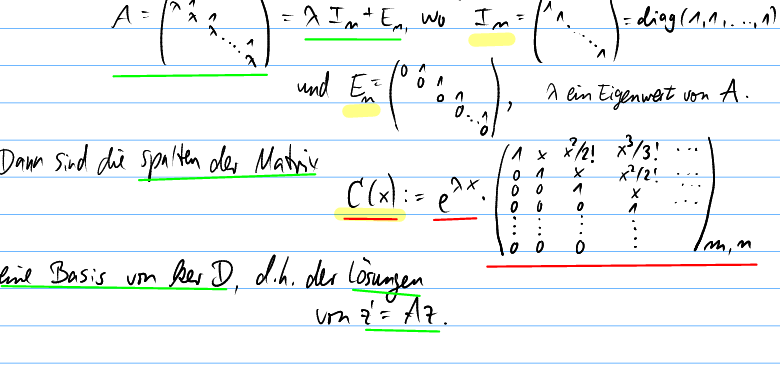
\includegraphics[width=10 cm,height=7cm]{bsp kap 23.12}
	\end{figure}\\ 
	\greenul{eine Basis von ker D}, d-h- der \greenul{Lösung} von \greenul{z'=Az}.\\
	\underline{Bew.:} Zu betrachten ist z'(x)=Az(x)=($\lambda I_n+E_n$)z(t).\\
	Mit einem noch zu bestimmenden Vektor \redul{$c(x)=\begin{pmatrix}
			c_1(x)\\
			\vdots\\
			c_n(x)
	\end{pmatrix}$} setzen wir an: \redul{z(x):=$e^{\lambda x}\cdot c(x)$}.\\
	Dies ergibt für alle x die zu erfüllende Gleichung \oraul{z'(x)}$=e^{\lambda x}\underbrace{(\lambda c(x)+c'(x))}_{\text{laut Produktregel}}\overset{!}{=}(\lambda I_n+E_n)e^{\lambda x}c(x)=e^{\lambda x}(\lambda c(x)+U_nc(x))\Leftrightarrow$ \oraul{$c'(x)=E_n c(x)$}.\\
	In Komponenten aufgeschrieben lautet die letzte Gleichung: \oraul{$c_i'(x)$}$\begin{cases}
		c_{i+1}(x);&1\textless n,\\
		0;&i=n
	\end{cases}$ \\
	und die \oraul{Spalten} der oben notierten Matrix C \oraul{sind offenbar Lösungen} dieser Gleichung. Da \oraul{C invertierbar} ist, sind sie \oraul{Linear unabhängig} und it Folgerung 23.8 also eine Basis.\\
	\\
	\textbf{23.13. \underline{Allgemeiner Fall:}} Sei A in (beliebiger) JNF gegeben, also als A=\begin{figure}[h]
		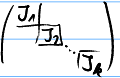
\includegraphics[width=2 cm,height=2cm]{bsp kap 23.13.1}
	\end{figure}\\ 
	mit \oraul{Jordan-Kästen $J_1,...,J_k$}. Zu jedem Jordan-Kasten $J_i$ bilde man entsprechend den Spezialfall \blueul{23.12} die \oraul{zugehörige Matrix $C_i(x)$} und ordne all diese Matrix an zur neuen Matrix\\
	\oraul{C(x)}=\begin{figure}[h]
		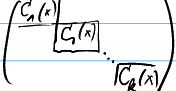
\includegraphics[width=2 cm,height=2cm]{bsp kap 23.13.2}
	\end{figure}.\\ 
	Dann sind die Spalten von C linear unabhängig und Lösungen von z'=Az, womit auch Satz \blueul{23.10.} gezeigt ist.\\
	\\
	\textbf{23.14. \underline{Bem.:}} Die DGL $u^{(n)} +a_{n-1}u^{(n-1)}+...+a_1u'+a_0u=f$ aus \blueul{an21} kann mir der Substitution $y_1=0,y_2=u'=y_1',y_3=u''=y_2',...,y_n=u^{n-1}=y_{n-1}'$ auf das System 1. Ordnung 
\end{document}